\begin{enumerate}[label=\thechapter.\arabic*,ref=\thechapter.\theenumi]
\item The outputs of four systems $\brak{S_{1} , S_{2} , S_{3},S_{4}}$ corresponding to the input signal $\sin\brak{t}$, for all time $t$ , are shown in the figure. Based on the given information, which of the four systems is/are definately NOT LTI(linear and time-invariant)? 
\begin{figure}[H]
    \resizebox{0.34\textwidth}{!}{\tikzset{
    block/.style = {draw, fill=white, rectangle, minimum height=3em, minimum width=3em}
}

\begin{tikzpicture}[auto, node distance=2cm,>=Latex]

    \node (input) {$\sin\brak{t}$};
    

    \node [block, right=of input] (s1) {$S_{1}$};
    
    \draw[dashed, draw=black] ($(s1.south west) + (-0.2,-0.2)$) rectangle ($(s1.north east) + (0.2,0.2)$);
    \draw [->] (input) -- (s1);
    \draw [->] (s1) -- ++(2,0) node[right]{$\sin\brak{-t}=-\sin\brak{t}$};
    \begin{scope}[yshift=-3cm]
        \node (input2) {$\sin\brak{t}$};
        \node [block, right=of input2] (s2) {$S_{2}$};
        \draw[dashed, draw=black] ($(s2.south west) + (-0.2,-0.2)$) rectangle ($(s2.north east) + (0.2,0.2)$);
        \draw [->] (input2) -- (s2);
        \draw [->] (s2) -- ++(2,0) node[right]{$\sin\brak{t+1}$};
    \end{scope}
    
    \begin{scope}[yshift=-6cm]
        \node (input3) {$\sin\brak{t}$};
        
   
        \node [block, right=of input3] (s3) {$S_{3}$};
        
   
        \draw[dashed, draw=black] ($(s3.south west) + (-0.2,-0.2)$) rectangle ($(s3.north east) + (0.2,0.2)$);
        

        \draw [->] (input3) -- (s3);
        \draw [->] (s3) -- ++(2,0) node[right]{$\sin\brak{2t}$};
    \end{scope}
       \begin{scope}[yshift=-9cm]
        \node (input3) {$\sin\brak{t}$};
        

        \node [block, right=of input3] (s3) {$S_{4}$};
        

        \draw[dashed, draw=black] ($(s3.south west) + (-0.2,-0.2)$) rectangle ($(s3.north east) + (0.2,0.2)$);
        

        \draw [->] (input3) -- (s3);
        \draw [->] (s3) -- ++(2,0) node[right]{$\sin^2\brak{t}$};
    \end{scope}
\end{tikzpicture}

}
    \caption{Block Diagram of Systems}
    \label{fig:question_fig_EC_Q46}
\end{figure}
\hfill(GATE22 EC Q46)\\
\solution
\iffalse
\let\negmedspace\undefined
\let\negthickspace\undefined
\documentclass[journal,12pt,twocolumn]{IEEEtran}
\usepackage{cite}
\usepackage{amsmath,amssymb,amsfonts,amsthm}
\usepackage{algorithmic}
\usepackage{graphicx}
\usepackage{textcomp}
\usepackage{xcolor}
\usepackage{txfonts}
\usepackage{listings}
\usepackage{enumitem}
\usepackage{mathtools}
\usepackage{float}
\usepackage{gensymb}
\usepackage{comment}
\usepackage[breaklinks=true]{hyperref}
\usepackage{tkz-euclide} 
\usepackage{listings}
\usepackage{gvv}                                        
\def\inputGnumericTable{}                                 
\usepackage[latin1]{inputenc}                                
\usepackage{color}                                            
\usepackage{array}          
\usetikzlibrary{positioning, arrows.meta,shapes}
\usepackage{longtable}                                       
\usepackage{calc}                                             
\usepackage{multirow}                                         
\usepackage{hhline}                                           
\usepackage{ifthen}                                           
\usepackage{lscape}
\usepackage{amsmath}
\newtheorem{theorem}{Theorem}[section]
\newtheorem{problem}{Problem}
\newtheorem{proposition}{Proposition}[section]
\newtheorem{lemma}{Lemma}[section]
\newtheorem{corollary}[theorem]{Corollary}
\newtheorem{example}{Example}[section]
\newtheorem{definition}[problem]{Definition}
\newcommand{\BEQA}{\begin{eqnarray}}
\newcommand{\EEQA}{\end{eqnarray}}
\newcommand{\define}{\stackrel{\triangle}{=}}
\theoremstyle{remark}
\newtheorem{rem}{Remark}
\begin{document}

\bibliographystyle{IEEEtran}
\title{GATE-EC-Q46}
\author{EE23BTECH11015 - DHANUSH V NAYAK$^{*}$% <-this % stops a space
}
\maketitle
\newpage
\bigskip
\renewcommand{\thefigure}{\arabic{figure}}
\renewcommand{\thetable}{\theenumi}
\textbf{Question:} The outputs of four systems $\brak{S_{1} , S_{2} , S_{3},S_{4}}$ corresponding to the input signal $\sin\brak{t}$, for all time $t$ , are shown in the figure. Based on the given information, which of the four systems is/are definately NOT LTI(linear and time-invariant)? 
\begin{figure}[H]
    \resizebox{0.34\textwidth}{!}{\tikzset{
    block/.style = {draw, fill=white, rectangle, minimum height=3em, minimum width=3em}
}

\begin{tikzpicture}[auto, node distance=2cm,>=Latex]

    \node (input) {$\sin\brak{t}$};
    

    \node [block, right=of input] (s1) {$S_{1}$};
    
    \draw[dashed, draw=black] ($(s1.south west) + (-0.2,-0.2)$) rectangle ($(s1.north east) + (0.2,0.2)$);
    \draw [->] (input) -- (s1);
    \draw [->] (s1) -- ++(2,0) node[right]{$\sin\brak{-t}=-\sin\brak{t}$};
    \begin{scope}[yshift=-3cm]
        \node (input2) {$\sin\brak{t}$};
        \node [block, right=of input2] (s2) {$S_{2}$};
        \draw[dashed, draw=black] ($(s2.south west) + (-0.2,-0.2)$) rectangle ($(s2.north east) + (0.2,0.2)$);
        \draw [->] (input2) -- (s2);
        \draw [->] (s2) -- ++(2,0) node[right]{$\sin\brak{t+1}$};
    \end{scope}
    
    \begin{scope}[yshift=-6cm]
        \node (input3) {$\sin\brak{t}$};
        
   
        \node [block, right=of input3] (s3) {$S_{3}$};
        
   
        \draw[dashed, draw=black] ($(s3.south west) + (-0.2,-0.2)$) rectangle ($(s3.north east) + (0.2,0.2)$);
        

        \draw [->] (input3) -- (s3);
        \draw [->] (s3) -- ++(2,0) node[right]{$\sin\brak{2t}$};
    \end{scope}
       \begin{scope}[yshift=-9cm]
        \node (input3) {$\sin\brak{t}$};
        

        \node [block, right=of input3] (s3) {$S_{4}$};
        

        \draw[dashed, draw=black] ($(s3.south west) + (-0.2,-0.2)$) rectangle ($(s3.north east) + (0.2,0.2)$);
        

        \draw [->] (input3) -- (s3);
        \draw [->] (s3) -- ++(2,0) node[right]{$\sin^2\brak{t}$};
    \end{scope}
\end{tikzpicture}

}
    \caption{Block Diagram of Systems}
    \label{fig:question_fig_EC_Q46}
\end{figure}
\hfill(GATE22 EC Q46)\\
\solution 
\fi
\begin{table}[H]
\centering
\renewcommand\thetable{1}
\setlength{\extrarowheight}{9pt}
\resizebox{0.4\textwidth}{!}{
\begin{tabular}{|c|c|c|}
\hline
\textbf{Parameter} & \textbf{Description} \\ \hline
$\brak{S_{1} , S_{2} , S_{3},S_{4}}$ & Systems Given  \\ \hline
$\sin\brak{t}$ & Input \\ \hline
$H\brak{\omega}$ & Transfer Function \\ \hline
$X\brak{\omega}$ & Fourier-Transform of input \\ \hline
$Y\brak{\omega}$ & Fourier-Transform of output \\ \hline
$\Phi(\omega)$ & Phase of Transfer Function \\ \hline
\end{tabular}}
\caption{Parameter Table}
\label{tab:gate_ec_Q46}
\end{table}

\begin{figure}[H]
    \resizebox{0.55\textwidth}{!}{\tikzset{
    block/.style = {draw, fill=white, rectangle, minimum height=3em, minimum width=3em}
}

\begin{tikzpicture}[auto, node distance=2cm,>=Latex]
    \node (input) {$x\brak{t}$};
    \node [block, right=of input] (s1) {$H\brak{\omega}$};
    \draw[dashed, draw=black] ($(s1.south west) + (-0.2,-0.2)$) rectangle ($(s1.north east) + (0.2,0.2)$);
    \draw [->] (input) -- (s1);
    \draw [->] (s1) -- ++(2,0) node[right]{$y\brak{t}$};
    \end{tikzpicture}

    }
    \caption{Block Diagram of LTI System}
    \label{fig:LTI_system_EC_q46}
\end{figure}
For an LTI system :
\begin{align}
    y(t)&=h(t)*x(t)\\
    Y\brak{\omega}&=H\brak{\omega}X\brak{\omega}
\end{align}
$H\brak{\omega}$ is a complex exponential :
\begin{align}
    H(j\omega)=\abs{H(j\omega)}e^{j\Phi\brak{\omega}}
\end{align}
$x(t)=\sin\brak{t}$, and $w_{o}=1 rad/sec$
\begin{align}
    X\brak{\omega}&=j\pi \brak{\delta(\omega+\omega_0)-\delta(\omega-\omega_0)}
\end{align}
Now,

\begin{align}
    Y\brak{\omega}=&\brak{\delta(\omega+\omega_0)-\delta(\omega-\omega_0)}\pi \abs{H\brak{\omega}}e^{j\Phi\brak{\omega}}\label{eq:gate22_ec_q46.1}
\end{align}

\begin{align}
    x\brak{t}\delta\brak{t-t_{o}} = x\brak{t_{0}}\delta\brak{t-t_{o}} \label{eq:gate_22_ec_delta_prop_1}
\end{align}
Using property \eqref{eq:gate_22_ec_delta_prop_1} in \eqref{eq:gate22_ec_q46.1} :
\begin{align}
    Y\brak{\omega}=&j\pi \abs{H(-\omega_0)}e^{j\Phi(-\omega_0)}\delta(\omega+\omega_0)\label{eq:gate_ec_q46.3} \\&- j\pi \abs{H\brak{\omega_0}}e^{j\Phi(j\omega_0)}\delta(\omega-\omega_0) \notag 
\end{align}
By definition of the Fourier transform,
\begin{align}
    X(\omega) &= \int_{-\infty}^{\infty} x\brak{t}e^{-j\omega t} \,dt \\
    X^*(\omega) &= \int_{-\infty}^{\infty} x^*(t)e^{j\omega t} \,dt \\
    X^*(-\omega) &= \int_{-\infty}^{\infty} x^*(t)e^{-j\omega t} \,dt\label{eq:gate_ec_q46.2}
\end{align}
For real-time domain signal :
\begin{align}
    x\brak{t} &= x^*\brak{t}
\end{align}
Therefore , from \eqref{eq:gate_ec_q46.2}:
\begin{align}
    X(\omega) =  X^*(-\omega) \label{eq:gate_ec_q46_conjsymm}
\end{align}
By \eqref{eq:gate_ec_q46_conjsymm} , Given $h(t)$ a real-time domain signal, $H\brak{\omega}$ is conjugate symmetric.
\begin{align}
    \abs{H\brak{\omega}}=\abs{H(-\omega)}\label{eq:gate_22_q46_conj_result1}\\
    \Phi(-\omega)=-\Phi\brak{\omega}\label{eq:gate_22_q46_conj_result2}
\end{align}
Therefore using \eqref{eq:gate_22_q46_conj_result1} and \eqref{eq:gate_22_q46_conj_result2} in \eqref{eq:gate_ec_q46.3},
 \begin{align}
    Y\brak{\omega}= j\pi \abs{H\brak{\omega_0}}\brak{e^{-j\Phi\brak{\omega_0}}\delta(\omega+\omega_0) - e^{j\Phi\brak{\omega_0}}\delta(\omega-\omega_0)}
\end{align}
Taking Inverse Fourier Transform, 
\begin{align}
    &\delta(\omega-\omega_0) \system{F} \frac{1}{2}e^{j\omega_0t}\\
     &\delta(\omega+\omega_0) \system{F} \frac{1}{2}e^{-j\omega_0t}\\
    &\implies y(t)=j\pi \abs{H\brak{\omega_0}}\frac{1}{2}\brak{e^{-j\brak{\omega_0t+\Phi\brak{\omega_0}}}-e^{j\brak{\omega_0t+\Phi\brak{\omega_0}}}}\\
    &\implies y(t) =\abs{H\brak{\omega_0}}\sin{\brak{\omega_0t+\Phi\brak{\omega_0}}} 
\end{align}
$w_{0} = 1$ rad/sec :
\begin{align}
    y(t) =\abs{H\brak{1}}\sin{\brak{t+\Phi\brak{1}}} \label{eq:gate_ec_q46_finaloutput}
\end{align}
From \eqref{eq:gate_ec_q46_finaloutput} we can see output cant have scaled frequency nor a squared output. But can have a shifted output or amplitude-scaled output. \\

So, $S_{3}$ and $S_{4}$ cannot be LTI system.
%\end{document}


\pagebreak

    \item The Fourier transform X\brak{j\omega} of the signal\\ $x(t)=\frac{t}{\brak{1+t^2}^2}$ is \rule{1.5cm}{0.15mm}.\hfill{GATE-2022-EC-15}
\begin{enumerate}
	\item[(A)] $\frac{\pi}{2j}\omega e^{-\abs{\omega}}$
	\item[(B)] $\frac{\pi}{2}\omega e^{-\abs{\omega}}$
	\item[(C)] $\frac{\pi}{2j}e^{-\abs{\omega}}$
	\item[(D)] $\frac{\pi}{2}e^{-\abs{\omega}}$
\end{enumerate}

\solution
\iffalse
\let\negmedspace\undefined
\let\negthickspace\undefined
\documentclass[journal,12pt,twocolumn]{IEEEtran}
\usepackage{cite}
\usepackage{amsmath,amssymb,amsfonts,amsthm}
\usepackage{algorithmic}
\usepackage{graphicx}
\usepackage{textcomp}
\usepackage{xcolor}
\usepackage{txfonts}
\usepackage{listings}
\usepackage{enumitem}
\usepackage{mathtools}
\usepackage{gensymb}
\usepackage{comment}
\usepackage[breaklinks=true]{hyperref}
\usepackage{tkz-euclide} 
\usepackage{listings}
\usepackage{gvv}                                        
\def\inputGnumericTable{}                                 
\usepackage[latin1]{inputenc}                                
\usepackage{color}                                            
\usepackage{array}                                            
\usepackage{longtable}                                       
\usepackage{calc}                                             
\usepackage{multirow}                                         
\usepackage{hhline}                                           
\usepackage{ifthen}                                           
\usepackage{lscape}
\usepackage[center]{caption} % center the captions to figure

\newtheorem{theorem}{Theorem}[section]
\newtheorem{problem}{Problem}
\newtheorem{proposition}{Proposition}[section]
\newtheorem{lemma}{Lemma}[section]
\newtheorem{corollary}[theorem]{Corollary}
\newtheorem{example}{Example}[section]
\newtheorem{definition}[problem]{Definition}
\newcommand{\BEQA}{\begin{eqnarray}}
\newcommand{\EEQA}{\end{eqnarray}}
\newcommand{\define}{\stackrel{\triangle}{=}}
\theoremstyle{remark}
\newtheorem{rem}{Remark}
\begin{document}

\newcolumntype{M}[1]{>{\centering\arraybackslash}m{#1}}
\newcolumntype{N}{@{}m{0pt}@{}}

\bibliographystyle{IEEEtran}
\vspace{3cm}

\title{GATE 2022 BM 14 Q} 
\author{ee23btech11223 - Soham Prabhakar More% <-this % stops a space
}
\maketitle
\newpage
\bigskip

\renewcommand{\thefigure}{\theenumi}
\renewcommand{\thetable}{\theenumi}

\bibliographystyle{IEEEtran}

\textbf{Question:} $x\brak{t}$ is a real continuous-time signal whose magnitude frequency response
$\abs{X\brak{j\Omega}}$ is shown below. After sampling $x\brak{t}$ at 100 $rad.s^{-1}$, the spectral point P
is down-converted to \rule{1cm}{0.15mm} $rad.s^{-1}$ in the spectrum of the sampled signal.
\hfill{(GATE 2022 BM 14 Q)}
\begin{figure}[h!]
    \renewcommand\thefigure{1}
    \centering
    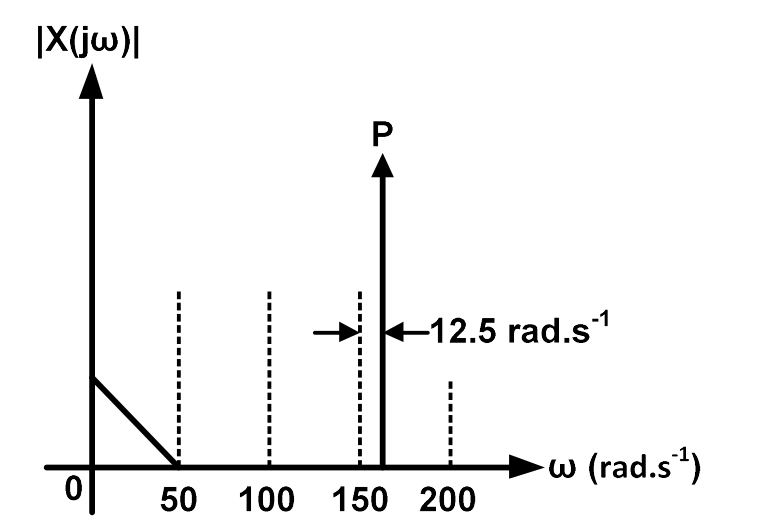
\includegraphics[width=\columnwidth]{2022/BM/14/figs/question.png}
    \caption[short]{Plot of $\abs{X\brak{j\omega}}$}
    \label{fig:2023.bm.14.img1}
\end{figure}

\solution
\fi
\begin{table}[ht]
    \renewcommand\thetable{1}
\begin{tabular}{|c|c|}
    \hline 
    \textbf{Parameter}&\textbf{Description} \\
    \hline
    $w\brak{t}$ & Sampling Function \\
    \hline
	$W\brak{j\omega}$ & Fourier Transform of $w\brak{t}$ \\
    \hline
    $x\brak{t}$ & Input Signal \\
    \hline
    $X\brak{j\omega}$ & Input Signal Frequency Spectrum \\
    \hline
    $x_s\brak{t}$ & Sampled Input Signal \\
    \hline
    $X_s\brak{j\omega}$ & Sampled Signal Frequency Spectrum \\
    \hline
\end{tabular}

\caption{Table of parameters}
\label{Table:1}


\end{table} \\
The sampling function is:
\begin{align}
    w(t) &= \sum_{k = -\infty}^{\infty}\delta\brak{t - \frac{2\pi k}{100}} \\
    W(j\omega) &= 100\sum_{k = -\infty}^{\infty}\delta\brak{j\brak{\omega - 100k}}
\end{align}
then the sampled function: 
\begin{align}
    x_s\brak{t} &= x\brak{t}w\brak{t} \\
    X_s\brak{j\omega} &= X\brak{j\omega} * W\brak{j\omega} \\
    X_s\brak{j\omega} &= \int_{-\infty}^{\infty}X\brak{j\theta}W\brak{j\brak{\omega - \theta}}d\theta \\
    X_s\brak{j\omega} &= 100\sum_{k = -\infty}^{\infty}\int_{-\infty}^{\infty}X\brak{j\theta}\delta\brak{j\brak{\omega - 100k - \theta}}d\theta \\
    X_s\brak{j\omega} &= 100\sum_{k = -\infty}^{\infty}X\brak{j\brak{\omega - 100k}} 
\end{align}
Thus, The down sampled point is at:
\begin{align}
    \omega &= \abs{162.5 - 100k}
\end{align}
where $k$ is the nearest integer to $\frac{162.5}{100}$, which is 2\\
Thus,
\begin{align}
    \omega = 37.5\,rad\,s^{-1}
\end{align}

\begin{figure}[h!]
    \renewcommand\thefigure{2}
    \centering
    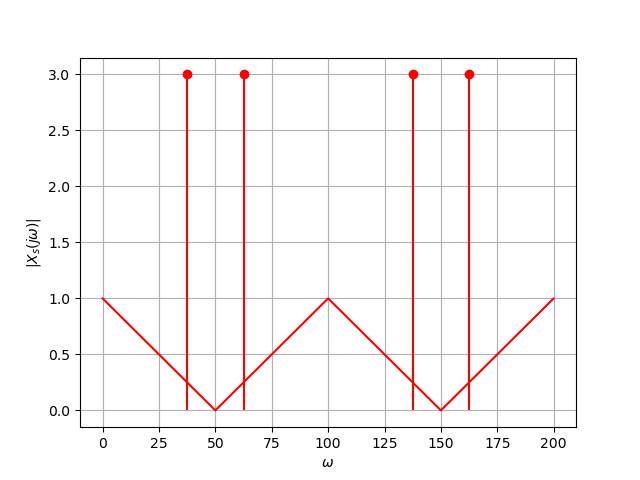
\includegraphics[width=\columnwidth]{2022/BM/14/figs/X_s.png}
    \caption[short]{Plot of $\abs{X_s\brak{j\omega}}$}
    \label{fig:2023.bm.14.img2}
\end{figure}

%\end{document}

\pagebreak

\item For a vector $\bar{x} = [x[0], x[1], \dots, x[7] ]$, the $8$-point discrete Fourier transform (DFT) is denoted by $\bar{X} = \text{DFT}(\bar{x}) = [X[0],X[1],\dots,X[7]]$, where
    \begin{align*}
    X[k] = \sum_{n=0}^{7}x[n]\exp\left(-j\frac{2\pi}{8}nk\right).
    \end{align*} 
    Here $j = \sqrt{-1}$. If $\bar{x} = [1,0,0,0,2,0,0,0]$ and $\bar{y} = \text{DFT}(\text{DFT}(\bar{x}))$, then the value of $y[0]$ is.\hfill{GATE-2022-EC-55}\\
    \solution
    \input{2022/EC/55/55.tex}
    \pagebreak
\item \textbf{Question:} An LTI system is shown in the figure where $$H\brak{s}= \frac{100}{s^2+0.1s+10}$$ The steady state output of the system for an input $x\brak{t}$ is given by $y\brak{t}=a+b\sin{\brak{10t+\theta}}$. The values of $'a'$ and $'b'$ are \\\\
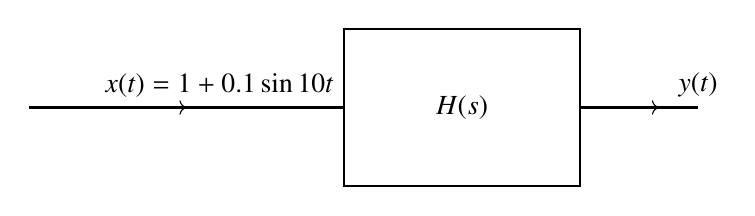
\begin{tikzpicture}
    \draw [thick, draw=black] (-2,-1) -- (2,-1) node[anchor=south east] {$x(t)=1+0.1\sin{\brak{10t}}$};
    \draw [thick,draw=black] (2,0) rectangle (5,-2) ;
    \draw [thick,draw=black] (5,-1) -- (6.5,-1) node[anchor=south] {$y(t)$};
    \draw [->] (-2,-1)--(0,-1);
    \draw [->] (5,-1)--(6,-1);
    \draw (3.5, -1) node[] {$H(s)$};
\end{tikzpicture}\\
\solution 
    \iffalse
\let\negmedspace\undefined
\let\negthickspace\undefined
\documentclass[journal,12pt,twocolumn]{IEEEtran}
\usepackage{cite}
\usepackage{amsmath,amssymb,amsfonts,amsthm}
\usepackage{algorithmic}
\usepackage{graphicx}
\usepackage{textcomp}
\usepackage{xcolor}
\usepackage{txfonts}
\usepackage{listings}
\usepackage{enumitem}
\usepackage{mathtools}
\usepackage{gensymb}
\usepackage{comment}
\usepackage[breaklinks=true]{hyperref}
\usepackage{tkz-euclide} 
\usepackage{listings}
\usepackage{gvv}                                        
\def\inputGnumericTable{}                                 
\usepackage[latin1]{inputenc}                                
\usepackage{color}                                            
\usepackage{array}                                            
\usepackage{longtable}                                       
\usepackage{calc}                                             
\usepackage{multirow}                                         
\usepackage{hhline}                                           
\usepackage{ifthen}                                           
\usepackage{lscape}
\usepackage[center]{caption} % center the captions to figure

\newtheorem{theorem}{Theorem}[section]
\newtheorem{problem}{Problem}
\newtheorem{proposition}{Proposition}[section]
\newtheorem{lemma}{Lemma}[section]
\newtheorem{corollary}[theorem]{Corollary}
\newtheorem{example}{Example}[section]
\newtheorem{definition}[problem]{Definition}
\newcommand{\BEQA}{\begin{eqnarray}}
\newcommand{\EEQA}{\end{eqnarray}}
\newcommand{\define}{\stackrel{\triangle}{=}}
\theoremstyle{remark}
\newtheorem{rem}{Remark}
\begin{document}

\newcolumntype{M}[1]{>{\centering\arraybackslash}m{#1}}
\newcolumntype{N}{@{}m{0pt}@{}}

\bibliographystyle{IEEEtran}
\vspace{3cm}

\title{GATE 2022 BM 14 Q} 
\author{ee23btech11223 - Soham Prabhakar More% <-this % stops a space
}
\maketitle
\newpage
\bigskip

\renewcommand{\thefigure}{\theenumi}
\renewcommand{\thetable}{\theenumi}

\bibliographystyle{IEEEtran}

\textbf{Question:} $x\brak{t}$ is a real continuous-time signal whose magnitude frequency response
$\abs{X\brak{j\Omega}}$ is shown below. After sampling $x\brak{t}$ at 100 $rad.s^{-1}$, the spectral point P
is down-converted to \rule{1cm}{0.15mm} $rad.s^{-1}$ in the spectrum of the sampled signal.
\hfill{(GATE 2022 BM 14 Q)}
\begin{figure}[h!]
    \renewcommand\thefigure{1}
    \centering
    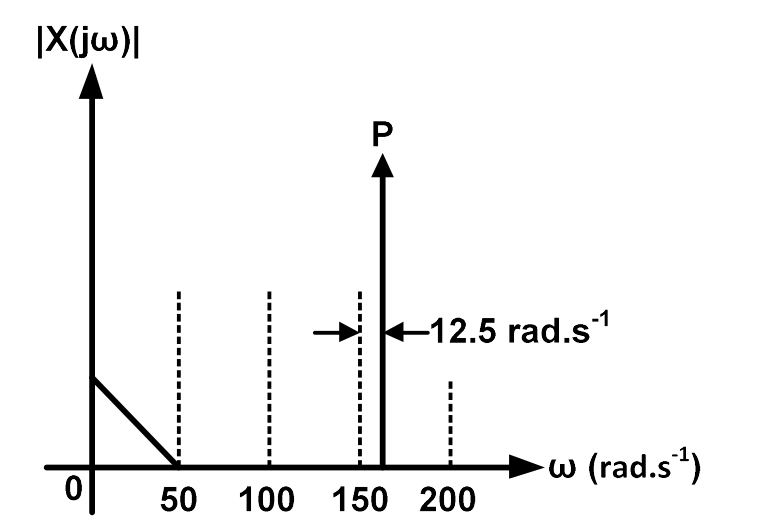
\includegraphics[width=\columnwidth]{2022/BM/14/figs/question.png}
    \caption[short]{Plot of $\abs{X\brak{j\omega}}$}
    \label{fig:2023.bm.14.img1}
\end{figure}

\solution
\fi
\begin{table}[ht]
    \renewcommand\thetable{1}
\begin{tabular}{|c|c|}
    \hline 
    \textbf{Parameter}&\textbf{Description} \\
    \hline
    $w\brak{t}$ & Sampling Function \\
    \hline
	$W\brak{j\omega}$ & Fourier Transform of $w\brak{t}$ \\
    \hline
    $x\brak{t}$ & Input Signal \\
    \hline
    $X\brak{j\omega}$ & Input Signal Frequency Spectrum \\
    \hline
    $x_s\brak{t}$ & Sampled Input Signal \\
    \hline
    $X_s\brak{j\omega}$ & Sampled Signal Frequency Spectrum \\
    \hline
\end{tabular}

\caption{Table of parameters}
\label{Table:1}


\end{table} \\
The sampling function is:
\begin{align}
    w(t) &= \sum_{k = -\infty}^{\infty}\delta\brak{t - \frac{2\pi k}{100}} \\
    W(j\omega) &= 100\sum_{k = -\infty}^{\infty}\delta\brak{j\brak{\omega - 100k}}
\end{align}
then the sampled function: 
\begin{align}
    x_s\brak{t} &= x\brak{t}w\brak{t} \\
    X_s\brak{j\omega} &= X\brak{j\omega} * W\brak{j\omega} \\
    X_s\brak{j\omega} &= \int_{-\infty}^{\infty}X\brak{j\theta}W\brak{j\brak{\omega - \theta}}d\theta \\
    X_s\brak{j\omega} &= 100\sum_{k = -\infty}^{\infty}\int_{-\infty}^{\infty}X\brak{j\theta}\delta\brak{j\brak{\omega - 100k - \theta}}d\theta \\
    X_s\brak{j\omega} &= 100\sum_{k = -\infty}^{\infty}X\brak{j\brak{\omega - 100k}} 
\end{align}
Thus, The down sampled point is at:
\begin{align}
    \omega &= \abs{162.5 - 100k}
\end{align}
where $k$ is the nearest integer to $\frac{162.5}{100}$, which is 2\\
Thus,
\begin{align}
    \omega = 37.5\,rad\,s^{-1}
\end{align}

\begin{figure}[h!]
    \renewcommand\thefigure{2}
    \centering
    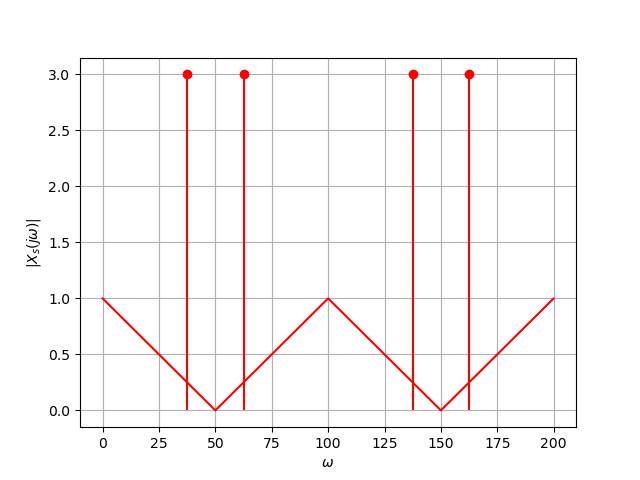
\includegraphics[width=\columnwidth]{2022/BM/14/figs/X_s.png}
    \caption[short]{Plot of $\abs{X_s\brak{j\omega}}$}
    \label{fig:2023.bm.14.img2}
\end{figure}

%\end{document}

\item A periodic function $f(x)$, with period 2, is defined as \\
   \begin{align}   
   f(x) =
   \begin{cases}
    -1-x & -1 \leq x<0 \\
     1-x &  0 <x \leq1 
   \end{cases}
   \end{align} 
   The Fourier series of this function contains \\
\begin{enumerate}[label=\Alph*.]
\item Both $\cos(n\pi x)$ and $sin(n\pi x)$ where n=1,2,3...
\item Only $\sin(n\pi x)$ where n=1,2,3...
\item Only $\cos(n\pi x)$ where n=1,2,3...
\item Only $\cos(2n\pi x)$ where n=1,2,3...  \hfill{GATE IN 2022 }
\end{enumerate} 

\solution
\input{2022/IN/13/g13.tex}

\end{enumerate}
